\chapter{Introduction}

This introduction provides an overview of the sustainability crisis in the fashion industry, introduces the concept of garment utility, and outlines the project focus.

\section{Sustainability Crisis in the Fashion Industry}
The fashion industry is a significant contributor to environmental degradation, second only to oil and mining \cite{charter_accelerating_2024}. Waste and inefficiencies are endemic over the entire lifecycle. 
\subsection{Sourcing and Processing}
The problem starts from yarn production whether harvesting natural materials like cotton or the production of synthetic fibres. For example, cotton farming uses pesticides and fertilisers that pollute soil and water, leading to disasters like the Aral Sea shrinkage \cite{noauthor_aral_nodate}, while polyester production emits greenhouse gases and microplastics, harming marine life and human health. Furthermore, dyeing and finishing processes in textile manufacturing release harmful chemicals into water bodies, affecting aquatic ecosystems and human health. According to the Ellen MacArthur Foundation, the industry is responsible for approximately 10\% of global carbon emissions and is the second-largest consumer of the world's water supply \cite{ellen_macarthur_foundation_new_2017}. Figure \ref{fig:resource_consumption} further quantifies the fashion industry's resource consumption.
\begin{figure} [H]
    \centering
    
\includegraphics[width=0.8\textwidth]{Images/sourcing donuts.png}
    \caption{Fashion industry's resource consumption \cite{charter_accelerating_2024}}
    \label{fig:resource_consumption}
\end{figure}
\subsection{Overproduction and Overconsumption}
The fast fashion business model results in a relentless cycle of overproduction and overconsumption. Brands rapidly produce large quantities of low-cost, low-quality garments to chase ever-changing trends and induce consumer demand. Estimates suggest that by 2050, annual garment production will reach a staggering 814 billion garments, with a cumulative total of over 9.5 trillion garments produced from now until then \cite{charter_accelerating_2024}. Social pressure to frequently update wardrobes undermines eco-conscious consumerism, fostering a throwaway culture, where clothing is discarded after only a few uses. Fabric wasteage increases with these production volumes. The resulting unsustainability is multi-dimensional: unsold inventory is discarded, consumers quickly dispose of their purchases, and cut losses are often not recycled. Pan describes this as a `wicked problem' plagued by short product life cycles and excessive waste \cite{charter_accelerating_2024}

To address unsustainable practices in the fashion industry, a holistic approach like Puglia et al.'s Circular Policy Canvas is essential. Focusing on early stages of the garment lifecycle can mitigate overproduction. Innovations at the production stage can influence consumer behavior by creating garments that are more appealing and longer-lasting. This can address gaps in the pre-consumption and consumption stages revealed in the Circular Policy Canvas \cite{puglia_circular_2024}.
% \begin{figure} [H]
%     \centering
%     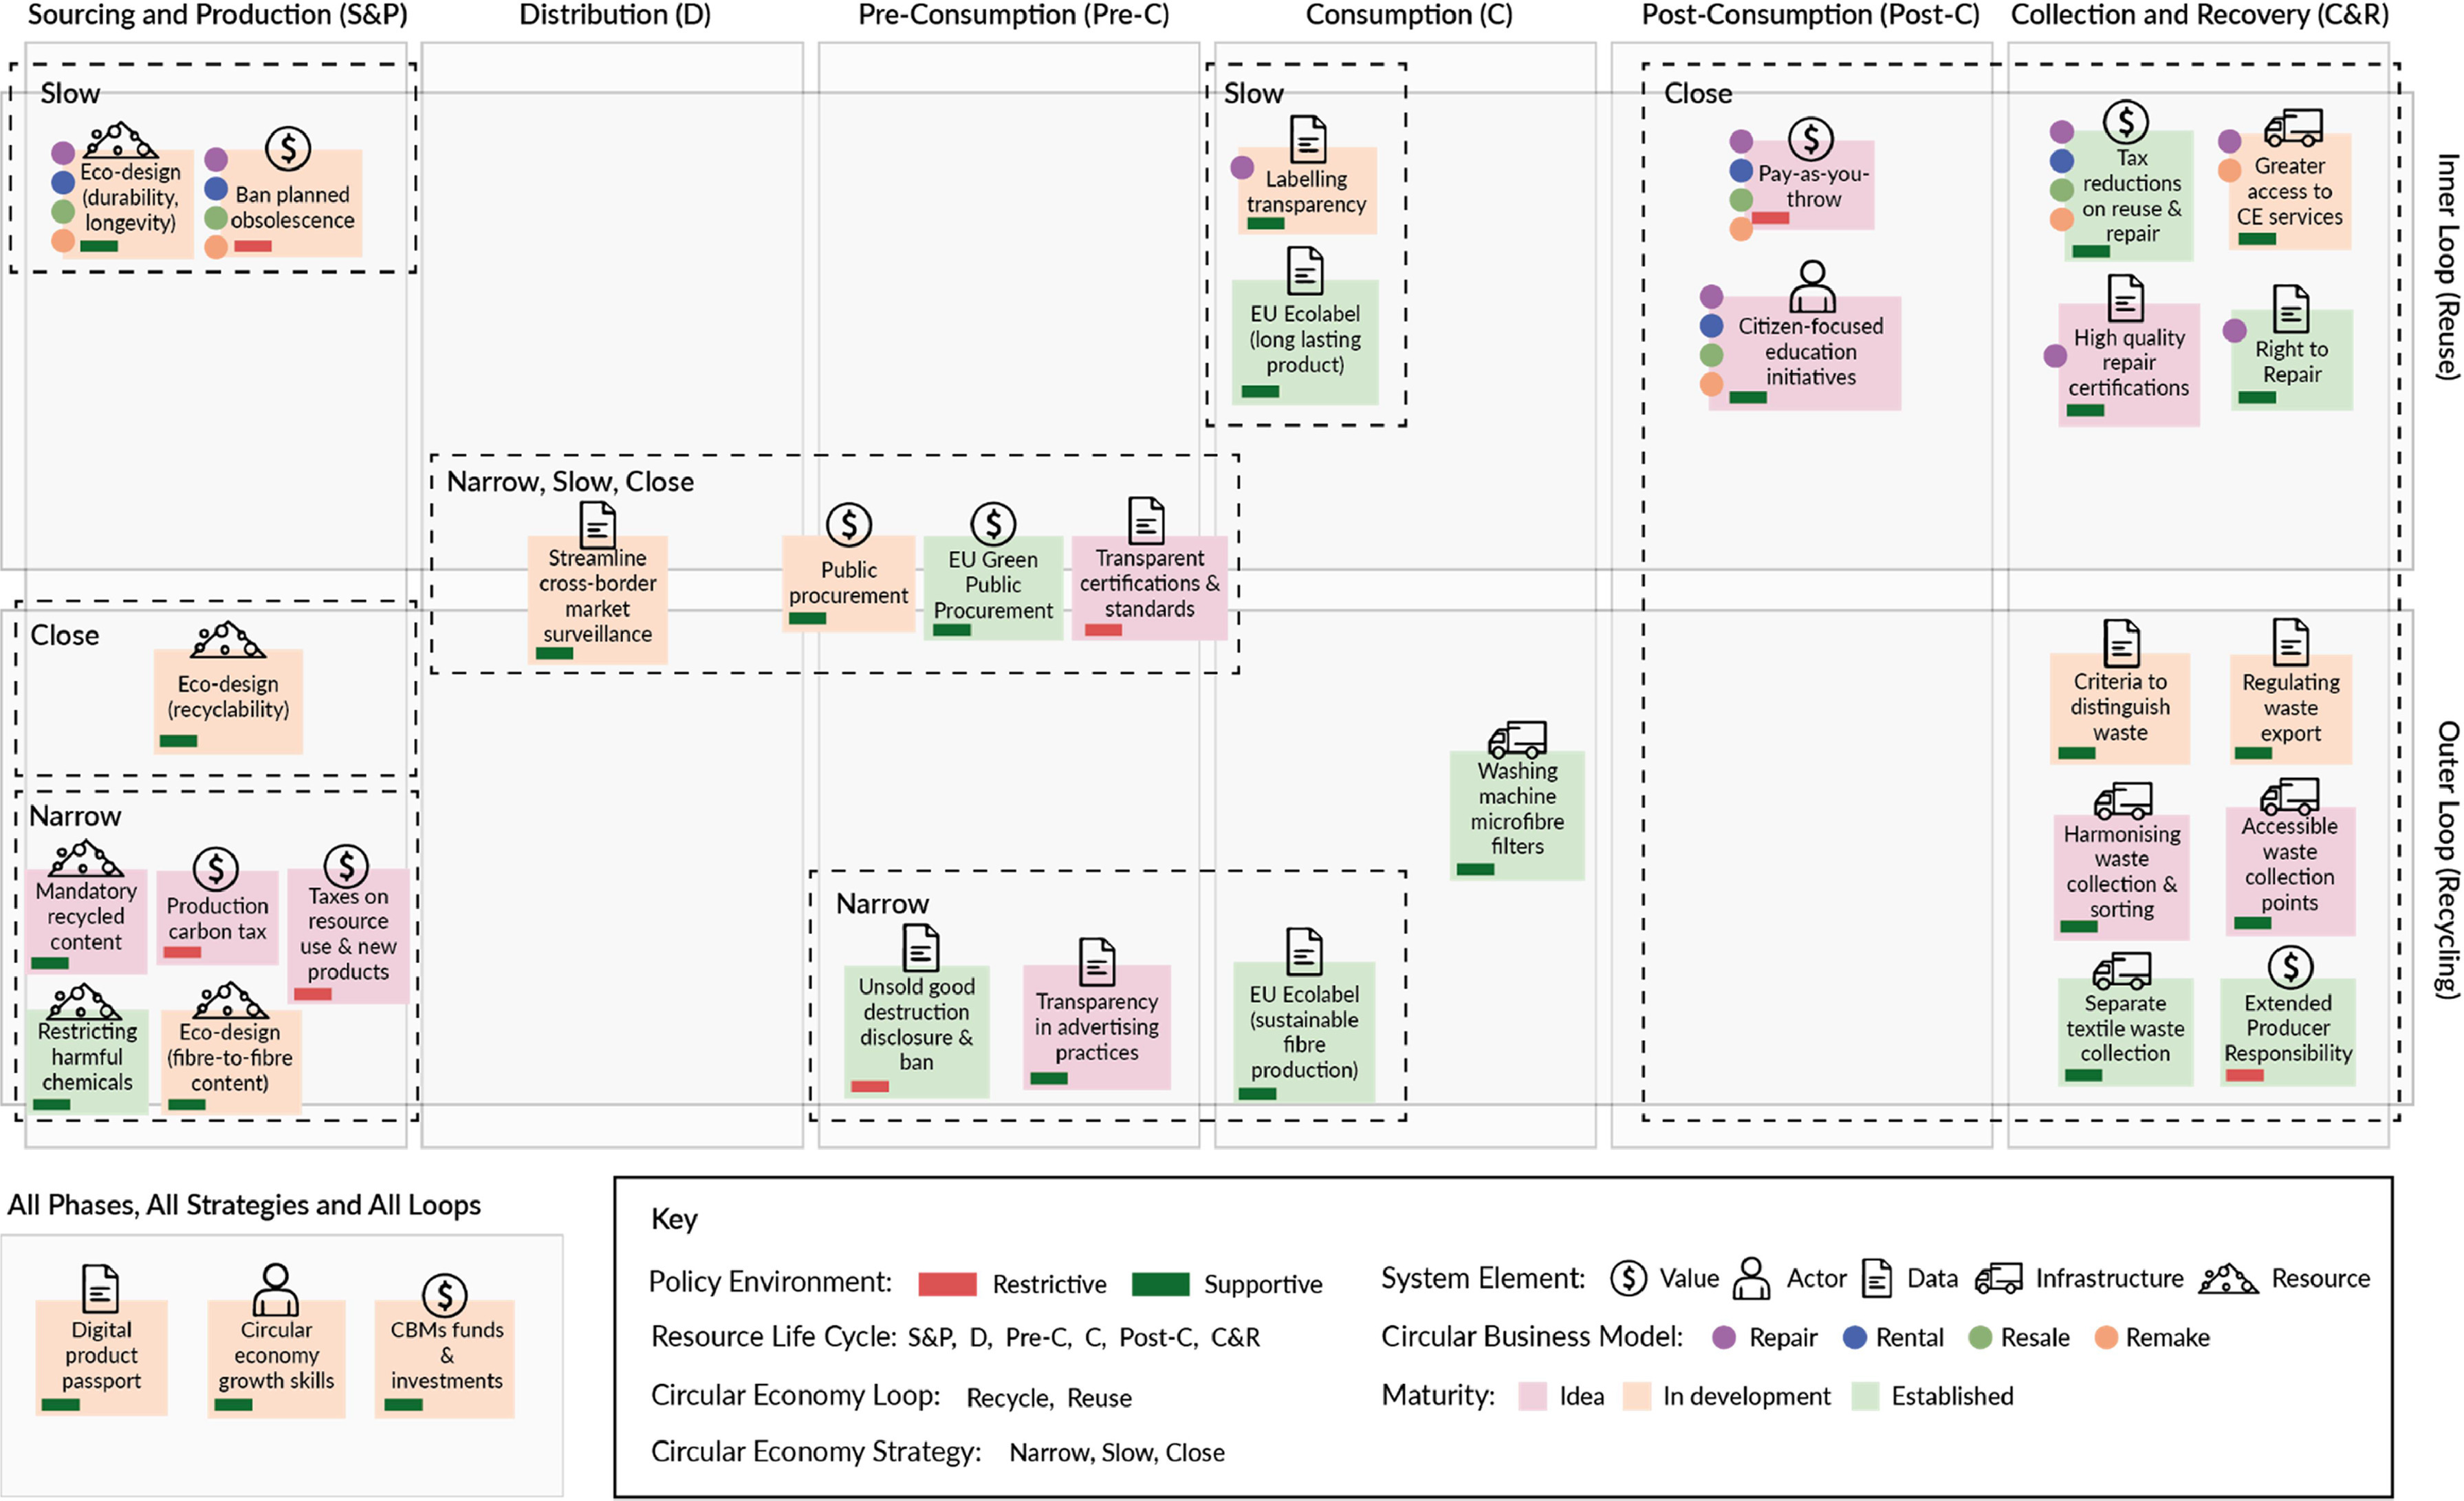
\includegraphics[width=\textwidth]{Images/circular policy canvas.png}
%     \caption{Circular Policy Canvas for the fashion industry \cite{puglia_circular_2024}}
%     \label{fig:circular_policy_canvas}
% \end{figure}

\section{Garment Utility}
Throughout this report, the author introduces and refers to the concept of \textit{garment utility}. Garment utility encompasses the functionality, durability, and versatility of a garment, as well as its aesthetic features that appeal to the user. It is influenced by the user's preferences, body shape, and lifestyle. Garment utility is a critical factor in determining a garment's value to the user, and attachment can significantly enhance the perceived value, as exemplified by the personal connection and increased value derived from tailoring.

\section{Project Focus}
Within the fashion supply chain, this project focuses on the garment manufacturing stage and how to reduce waste both pre- and post-sale. This is a question of material efficiency but also of what makes a garment desirable and why people might value it on an individual level . 

The project will explore the concept of `zero waste patterns' and how they can be parameterised based on individual body measurements. The aim is to create designs that are both sustainable and desirable, increasing garment utility by recouping fabric cut loss introduce by adding fit. This will involve exploring the principles of zero waste pattern making, bespoke clothing, and garment utility, and how these concepts can be integrated into the design process to enhance both sustainability and consumer attachment to the garments.

Make 2nd paragraph more concrete and specific to the project and its aims and how it will be eval'd

Within the fashion supply chain, this project focuses on the garment manufacturing stage and how to reduce waste in production and post-sale. It targets material efficiency and also what makes a garment desirable and valuable to consumers on a personal level \cite{black_sustainable_2013}. 

It will explore one `zero-waste' pattern' and how it can be parameterised based on individual body measurements. These bespoke designs will be verified virtually in commercial 3D software and tested in a workshop setting as well as on publicly available data sets. The goal is to make designs that are both sustainable and desirable, increase garment utility by recouping any fabric cut loss. The focus is on how these concepts can be integrated into the design process to enhance both sustainability and consumer customization of the garments.
